 \documentclass{article}
\usepackage[utf8]{inputenc}
\usepackage[shortlabels]{enumitem}
\usepackage{amsmath} 
\usepackage{gensymb}
\usepackage{geometry}
\usepackage{listings}
\usepackage{xcolor}
\usepackage{pgfplots}
\usepackage{pgfplotstable}
\pgfplotsset{compat=1.7}
\usepackage{tikz}
\definecolor{codegreen}{rgb}{0,0.6,0}
\definecolor{codegray}{rgb}{0.5,0.5,0.5}
\definecolor{codepurple}{rgb}{0.58,0,0.82}
\definecolor{backcolour}{rgb}{0.95,0.95,0.92}
\lstdefinestyle{mystyle}{
    backgroundcolor=\color{backcolour},   
    commentstyle=\color{codegreen},
    keywordstyle=\color{magenta},
    numberstyle=\tiny\color{codegray},
    stringstyle=\color{codepurple},
    basicstyle=\ttfamily\footnotesize,
    breakatwhitespace=false,         
    breaklines=true,                 
    captionpos=b,                    
    keepspaces=true,                 
    numbers=left,                    
    numbersep=5pt,                  
    showspaces=false,                
    showstringspaces=false,
    showtabs=false,                  
    tabsize=2
}

\lstset{style=mystyle}
\geometry{
 a4paper,
 total={170mm,257mm},
 left=20mm,
 top=20mm,
}

\title{Assignment: Iterative Process}
\author{Andy Yan}
\date{September 2022}

\begin{document}

\maketitle

\section{Question}

The equation \(x^2 - x - 2 = 0\) may be solved by using iterative process if you write it as \(x_{n+1}=x_n^2 - 2\)
When you reach a point where \(x_n+1 = x_n\), you have solved the equation. However, this process may not
work because it is very sensitive to the initial value.
\[\]
In this assignment, we will explore this sensitivity on initial value of the nonlinear system. Do the following:
\begin{enumerate}
\item  Try the initial value \(x_1 = 0\). See if this leads to a solution
\item  Try the initial value \(x_1 = 1\). See if this leads to a solution
\item  Try the initial value \(x_1 = 0.5\). See if this leads to a solution
\item  Try the initial value \(x_1 = 0.2\). See if this leads to a solution
\end{enumerate}

Note: you need to come at least x10 to assume if it leads to a solution or not.
\section{Problem Approach}
In order to solve an equation using the iterative process, we begin with an initial value \(x_1\).
\[x_2 = f(x_1)\]
\[x_3 = f(x_2) = f(f(x_1))\]
\[x_4 = f(x_3) = f(f(x_2)) = f(f(f(x_1)))\]
\[x_{n+1} = f(x_n) = f(f(x_{n-1})) = f(f(f(...\]
To compute the value of \(x_{n+1}\), we must compute all the values before it, since each value is calculated based on the last value. At an unknown value of \(x_n\) , \(x_{n+1}\) will provide us with a solution of the equation. However, this process is tedious and isn't guaranteed to work. So let us use a program to do it for us.
\section{Programming}
Lets declare the major variables that we will be needing to use:
\begin{itemize}
\item \textbf{init} : double (initial value \(x_1\))
\item \textbf{seq} : double[] (a list that will store values \(x_1\) to \(x_{n+1}\)
\end{itemize}
We will be using the double variable type to store decimals, and a double array so we can store the term of the value in the sequence. So,
\[init = x_1\]
\[seq[] = {x_1, x_2,...,x_{n+1}}\]
The value of \textbf{init} will be inputted and \textbf{seq}[n] will return the \(x_n\) or \textit{nth} term in the sequence. Using a for-loop, the program will return the value of \textbf{seq}[i] or \(x_i\) until the 10th term is reached. 
\[ \]
Here is the C++ program. 

\begin{lstlisting}[language=C++]
#include <bits/stdc++.h>
using namespace std;
int main() {
    double init, seq[11]; 
    cin>>init;
    seq[1]=init;
    for(int i = 2;i<=10;i++){
        seq[i]=seq[i-1] * seq[i-1] - 2;
        cout<<"n = "<<i<<" "<<seq[i]<<"\n";
    }
}
\end{lstlisting}
\section{Data}
Using the program above we can easily compute the first 10 terms of the sequence given any initial value \(x_1\). 
\begin{center}
\begin{tabular}{|c | c c c c|} 
 \hline
   &\(x_1 = 0\)&\(x_1 = 1\)&\(x_1 = 0.5\)&\(x_1 = 0.2\)\\ [1ex] 
 \hline
 \(n = 2\) & -2 & -1 & -1.75 & -1.96\\ 
 \hline
 \(n = 3\) & 2 & -1 & 1.0625 & 1.8416\\
 \hline
 \(n = 4\) & 2 & -1 & -0.871094 & 1.39149\\
 \hline
 \(n = 5\) & 2 & -1 & -1.2412 & -0.063754\\
 \hline
 \(n = 6\) & 2 & -1 & -0.459433 & -1.99594\\
 \hline
 \(n = 7\) & 2 & -1 & -1.78892 & 1.98376\\ 
 \hline
 \(n = 8\) & 2 & -1 & 1.20024 & 1.9353\\
 \hline
 \(n = 9\) & 2 & -1 & -0.559427 & 1.74537\\
 \hline
 \(n = 10\) & 2 & -1 & -1.68704 & 1.04633\\
 \hline
\end{tabular}
\end{center}

\section{Analysis}
Now we are given a number of values that could potentially be a solution to the equation \(x^2 - x - 2 = 0\). Let us start with our initial values:
\[(0)^2 - (0) - 2 = -2 \neq 0\]
\[(1)^2 - (1) - 2 = -2 \neq 0\]
\[(0.5)^2 - (0.5) - 2 = -2.25 \neq 0\]
\[(0.2)^2 - (0.2) - 2 = -2.16 \neq 0\]
As we can observe, none of these are solutions. We can try our values when \(n = 2\).
\[(2)^2 - (2) - 2 = 0\]
\[(-1)^2 - (-1) - 2 = 0\]
\[(0.5)^2 - (0.5) - 2 \neq 0\]
\[(0.2)^2 - (0.2) - 2 \neq 0\]
Now we have found our two solutions 2 and -1 to our quadratic equation. The initial values \(x_1 = 0,1\) do converge to a solution. However, our other two initial values do not converge to 2 or -1 within the 10 terms. 
\section{Graphs}
For our graphs, we can alter our program to compute more values of n to provide a better image. We will represent the \(x_n\) value on the y-axis and the n value on the x-axis. 
\[\]
\[\]
\[\]
\[\]
\[\]
\textbf{Graph 1}: inital value \(x_1 = 0.5\)

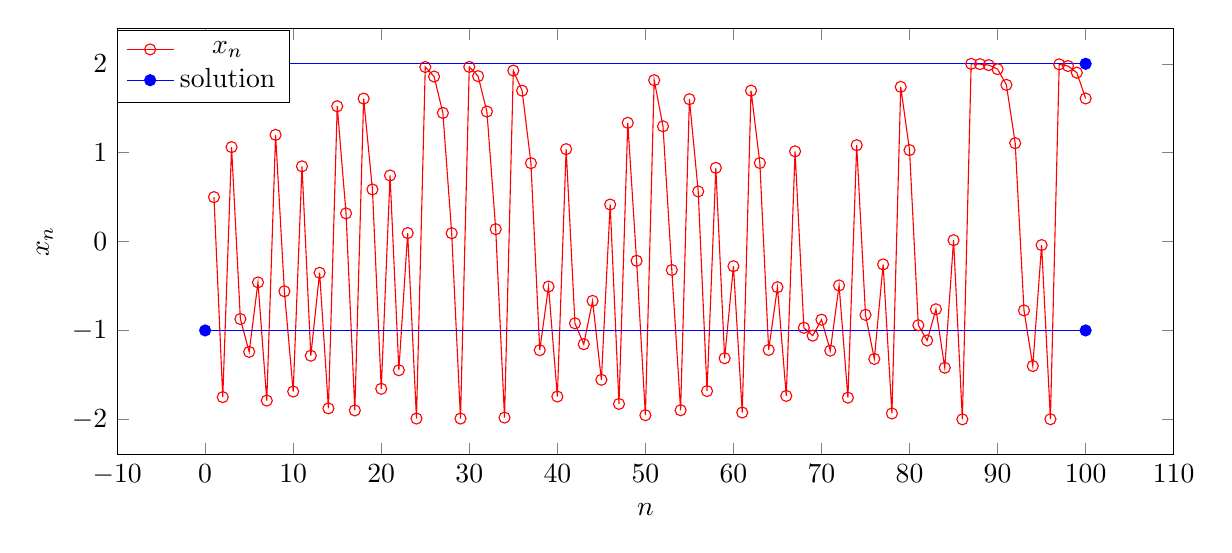
\begin{tikzpicture}
\begin{axis}[
	xlabel=\(n\),
	ylabel=\(x_n\),
	width=15cm,height=7cm,
    legend style={at={(0.0,.91)},anchor=west}
    ]

% Add values and attributes for the first plot
\addplot[color=red,mark=o] coordinates {
	(1, 0.5)
(2, -1.75)
(3, 1.0625)
(4, -0.871094)
(5, -1.2412)
(6, -0.459433)
(7, -1.78892)
(8, 1.20024)
(9, -0.559427)
(10, -1.68704)
(11, 0.846107)
(12, -1.2841)
(13, -0.35108)
(14, -1.87674)
(15, 1.52216)
(16, 0.316982)
(17, -1.89952)
(18, 1.60819)
(19, 0.586263)
(20, -1.6563)
(21, 0.743315)
(22, -1.44748)
(23, 0.0952068)
(24, -1.99094)
(25, 1.96382)
(26, 1.85661)
(27, 1.44699)
(28, 0.0937885)
(29, -1.9912)
(30, 1.96489)
(31, 1.8608)
(32, 1.46258)
(33, 0.139147)
(34, -1.98064)
(35, 1.92293)
(36, 1.69765)
(37, 0.882007)
(38, -1.22206)
(39, -0.50656)
(40, -1.7434)
(41, 1.03943)
(42, -0.919576)
(43, -1.15438)
(44, -0.667408)
(45, -1.55457)
(46, 0.416678)
(47, -1.82638)
(48, 1.33566)
(49, -0.216005)
(50, -1.95334)
(51, 1.81554)
(52, 1.2962)
(53, -0.319863)
(54, -1.89769)
(55, 1.60122)
(56, 0.563903)
(57, -1.68201)
(58, 0.829169)
(59, -1.31248)
(60, -0.277399)
(61, -1.92305)
(62, 1.69812)
(63, 0.883617)
(64, -1.21922)
(65, -0.513499)
(66, -1.73632)
(67, 1.0148)
(68, -0.970179)
(69, -1.05875)
(70, -0.879041)
(71, -1.22729)
(72, -0.493767)
(73, -1.75619)
(74, 1.08422)
(75, -0.824469)
(76, -1.32025)
(77, -0.256937)
(78, -1.93398)
(79, 1.74029)
(80, 1.02862)
(81, -0.941946)
(82, -1.11274)
(83, -0.761813)
(84, -1.41964)
(85, 0.0153784)
(86, -1.99976)
(87, 1.99905)
(88, 1.99622)
(89, 1.98488)
(90, 1.93976)
(91, 1.76267)
(92, 1.10701)
(93, -0.774529)
(94, -1.40011)
(95, -0.0397045)
(96, -1.99842)
(97, 1.9937)
(98, 1.97483)
(99, 1.89994)
(100, 1.60977)

};
\addplot[color=blue,mark=*] coordinates {
	(0, 2)
	(100,2)
};
\addplot[color=blue,mark=*] coordinates {
	(0, -1)
	(100,-1)
};

\legend{\(x_n\),solution}
\end{axis}
\end{tikzpicture}

\textbf{Graph 2}: inital value \(x_1 = 0.2\)

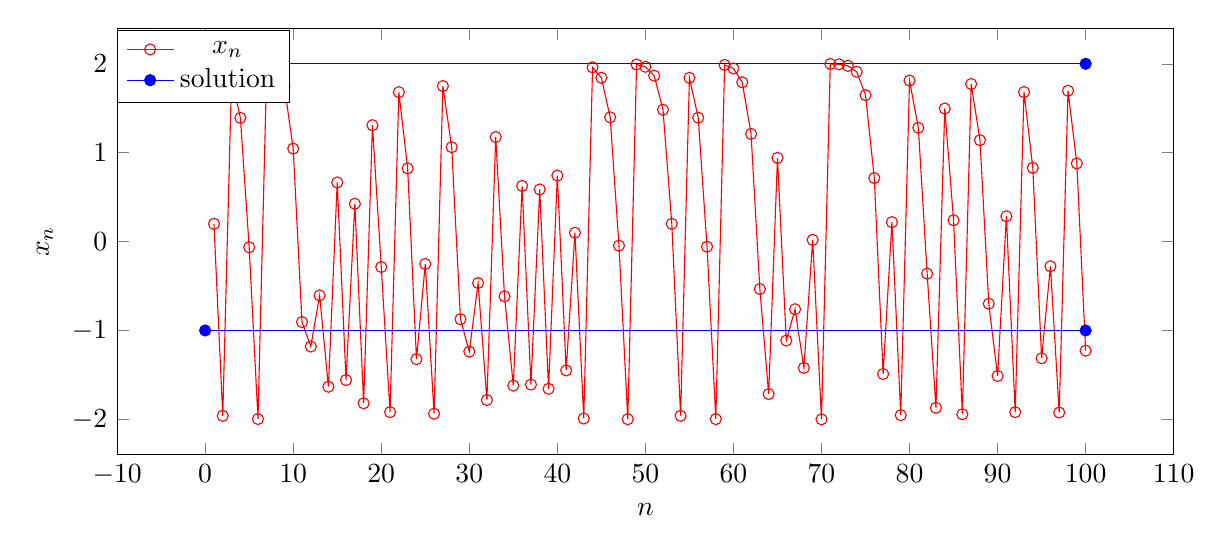
\begin{tikzpicture}
\begin{axis}[
	xlabel=\(n\),
	ylabel=\(x_n\),
	width=15cm,height=7cm,
    legend style={at={(0.0,.91)},anchor=west}
    ]

% Add values and attributes for the first plot
\addplot[color=red,mark=o] coordinates {
	(1, 0.2)
(2, -1.96)
(3, 1.8416)
(4, 1.39149)
(5, -0.063754)
(6, -1.99594)
(7, 1.98376)
(8, 1.9353)
(9, 1.74537)
(10, 1.04633)
(11, -0.905198)
(12, -1.18062)
(13, -0.606146)
(14, -1.63259)
(15, 0.66534)
(16, -1.55732)
(17, 0.425256)
(18, -1.81916)
(19, 1.30933)
(20, -0.285644)
(21, -1.91841)
(22, 1.68029)
(23, 0.823363)
(24, -1.32207)
(25, -0.252123)
(26, -1.93643)
(27, 1.74978)
(28, 1.06172)
(29, -0.87276)
(30, -1.23829)
(31, -0.46664)
(32, -1.78225)
(33, 1.17641)
(34, -0.616069)
(35, -1.62046)
(36, 0.625885)
(37, -1.60827)
(38, 0.586524)
(39, -1.65599)
(40, 0.742301)
(41, -1.44899)
(42, 0.0995699)
(43, -1.99009)
(44, 1.96044)
(45, 1.84333)
(46, 1.39787)
(47, -0.0459592)
(48, -1.99789)
(49, 1.99156)
(50, 1.96629)
(51, 1.86631)
(52, 1.48311)
(53, 0.199612)
(54, -1.96015)
(55, 1.84221)
(56, 1.39373)
(57, -0.0575209)
(58, -1.99669)
(59, 1.98678)
(60, 1.94728)
(61, 1.7919)
(62, 1.2109)
(63, -0.533709)
(64, -1.71515)
(65, 0.941755)
(66, -1.1131)
(67, -0.761014)
(68, -1.42086)
(69, 0.0188352)
(70, -1.99965)
(71, 1.99858)
(72, 1.99433)
(73, 1.97734)
(74, 1.90986)
(75, 1.64757)
(76, 0.714502)
(77, -1.48949)
(78, 0.218573)
(79, -1.95223)
(80, 1.81119)
(81, 1.28039)
(82, -0.360595)
(83, -1.86997)
(84, 1.49679)
(85, 0.240389)
(86, -1.94221)
(87, 1.77219)
(88, 1.14067)
(89, -0.69888)
(90, -1.51157)
(91, 0.284835)
(92, -1.91887)
(93, 1.68206)
(94, 0.829318)
(95, -1.31223)
(96, -0.278048)
(97, -1.92269)
(98, 1.69673)
(99, 0.878905)
(100, -1.22753)

};
\addplot[color=blue,mark=*] coordinates {
	(0, 2)
	(100,2)
};
\addplot[color=blue,mark=*] coordinates {
	(0, -1)
	(100,-1)
};

\legend{\(x_n\),solution}
\end{axis}
\end{tikzpicture}

We still observe that the initial values \(x_1 = 0.5,0.2\) don't converge to 2 or -1. We can also observe oscillating behaviors for initial values \(x_1 = 0.5,0.2\), and we know that oscillating functions don't converge to a value when approaching infinity. Hence, we can conclude that initial values \(x_1 = 0.5,0.2\) \textbf{don't converge to a solution.}

\section{Optional}

Lets try to compute  up to \(x_{1000}\) with the initial value 0.3.

\textbf{Graph 3}: inital value \(x_1 = 0.3\)

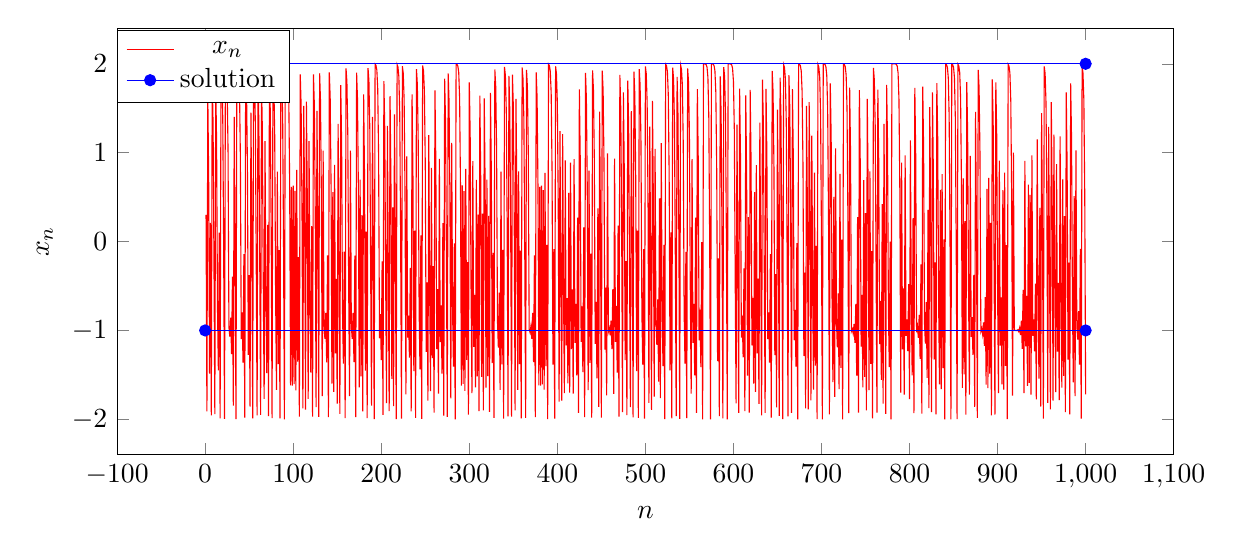
\begin{tikzpicture}
\begin{axis}[
	xlabel=\(n\),
	ylabel=\(x_n\),
	width=15cm,height=7cm,
    legend style={at={(0.0,.91)},anchor=west}
    ]

% Add values and attributes for the first plot
\addplot[color=red,mark=.] coordinates {
	(1, 0.3)
(2, -1.91)
(3, 1.6481)
(4, 0.716234)
(5, -1.48701)
(6, 0.211197)
(7, -1.9554)
(8, 1.82357)
(9, 1.32542)
(10, -0.243267)
(11, -1.94082)
(12, 1.76679)
(13, 1.12153)
(14, -0.742164)
(15, -1.44919)
(16, 0.100158)
(17, -1.98997)
(18, 1.95997)
(19, 1.8415)
(20, 1.39111)
(21, -0.0648034)
(22, -1.9958)
(23, 1.98322)
(24, 1.93316)
(25, 1.73711)
(26, 1.01755)
(27, -0.964598)
(28, -1.06955)
(29, -0.85606)
(30, -1.26716)
(31, -0.3943)
(32, -1.84453)
(33, 1.40228)
(34, -0.033608)
(35, -1.99887)
(36, 1.99548)
(37, 1.98195)
(38, 1.92814)
(39, 1.71772)
(40, 0.950574)
(41, -1.09641)
(42, -0.797889)
(43, -1.36337)
(44, -0.141213)
(45, -1.98006)
(46, 1.92063)
(47, 1.68883)
(48, 0.85215)
(49, -1.27384)
(50, -0.37733)
(51, -1.85762)
(52, 1.45076)
(53, 0.104705)
(54, -1.98904)
(55, 1.95627)
(56, 1.82698)
(57, 1.33786)
(58, -0.210127)
(59, -1.95585)
(60, 1.82534)
(61, 1.33185)
(62, -0.226175)
(63, -1.94884)
(64, 1.798)
(65, 1.23279)
(66, -0.480227)
(67, -1.76938)
(68, 1.13071)
(69, -0.721487)
(70, -1.47946)
(71, 0.188794)
(72, -1.96436)
(73, 1.8587)
(74, 1.45476)
(75, 0.116326)
(76, -1.98647)
(77, 1.94606)
(78, 1.78713)
(79, 1.19385)
(80, -0.574732)
(81, -1.66968)
(82, 0.787843)
(83, -1.3793)
(84, -0.0975227)
(85, -1.99049)
(86, 1.96205)
(87, 1.84963)
(88, 1.42114)
(89, 0.0196285)
(90, -1.99961)
(91, 1.99846)
(92, 1.99384)
(93, 1.97539)
(94, 1.90217)
(95, 1.61826)
(96, 0.618779)
(97, -1.61711)
(98, 0.615051)
(99, -1.62171)
(100, 0.62995)
(101, -1.60316)
(102, 0.57013)
(103, -1.67495)
(104, 0.805463)
(105, -1.35123)
(106, -0.174179)
(107, -1.96966)
(108, 1.87957)
(109, 1.53277)
(110, 0.349395)
(111, -1.87792)
(112, 1.5266)
(113, 0.330493)
(114, -1.89077)
(115, 1.57503)
(116, 0.480712)
(117, -1.76892)
(118, 1.12906)
(119, -0.725213)
(120, -1.47407)
(121, 0.172872)
(122, -1.97012)
(123, 1.88135)
(124, 1.5395)
(125, 0.370047)
(126, -1.86307)
(127, 1.47101)
(128, 0.163876)
(129, -1.97314)
(130, 1.8933)
(131, 1.58459)
(132, 0.51091)
(133, -1.73897)
(134, 1.02402)
(135, -0.951384)
(136, -1.09487)
(137, -0.801262)
(138, -1.35798)
(139, -0.155894)
(140, -1.9757)
(141, 1.90338)
(142, 1.62285)
(143, 0.633645)
(144, -1.59849)
(145, 0.555184)
(146, -1.69177)
(147, 0.862088)
(148, -1.2568)
(149, -0.420442)
(150, -1.82323)
(151, 1.32416)
(152, -0.246594)
(153, -1.93919)
(154, 1.76046)
(155, 1.09923)
(156, -0.791692)
(157, -1.37322)
(158, -0.114258)
(159, -1.98695)
(160, 1.94795)
(161, 1.79451)
(162, 1.22028)
(163, -0.510928)
(164, -1.73895)
(165, 1.02396)
(166, -0.951511)
(167, -1.09463)
(168, -0.801793)
(169, -1.35713)
(170, -0.158205)
(171, -1.97497)
(172, 1.90051)
(173, 1.61194)
(174, 0.598366)
(175, -1.64196)
(176, 0.696028)
(177, -1.51555)
(178, 0.296879)
(179, -1.91186)
(180, 1.65522)
(181, 0.739754)
(182, -1.45276)
(183, 0.110521)
(184, -1.98779)
(185, 1.95129)
(186, 1.80753)
(187, 1.26717)
(188, -0.39429)
(189, -1.84454)
(190, 1.40231)
(191, -0.033528)
(192, -1.99888)
(193, 1.9955)
(194, 1.98204)
(195, 1.92848)
(196, 1.71903)
(197, 0.955078)
(198, -1.08783)
(199, -0.816635)
(200, -1.33311)
(201, -0.222825)
(202, -1.95035)
(203, 1.80386)
(204, 1.25392)
(205, -0.427696)
(206, -1.81708)
(207, 1.30176)
(208, -0.30541)
(209, -1.90672)
(210, 1.6356)
(211, 0.675186)
(212, -1.54412)
(213, 0.384317)
(214, -1.8523)
(215, 1.43102)
(216, 0.0478102)
(217, -1.99771)
(218, 1.99086)
(219, 1.96353)
(220, 1.85546)
(221, 1.44271)
(222, 0.0814241)
(223, -1.99337)
(224, 1.97352)
(225, 1.8948)
(226, 1.59026)
(227, 0.528931)
(228, -1.72023)
(229, 0.959197)
(230, -1.07994)
(231, -0.833727)
(232, -1.3049)
(233, -0.297237)
(234, -1.91165)
(235, 1.65441)
(236, 0.737061)
(237, -1.45674)
(238, 0.122096)
(239, -1.98509)
(240, 1.94059)
(241, 1.7659)
(242, 1.11841)
(243, -0.749169)
(244, -1.43875)
(245, 0.0699905)
(246, -1.9951)
(247, 1.98043)
(248, 1.9221)
(249, 1.69447)
(250, 0.871226)
(251, -1.24096)
(252, -0.460006)
(253, -1.78839)
(254, 1.19835)
(255, -0.563948)
(256, -1.68196)
(257, 0.828999)
(258, -1.31276)
(259, -0.27666)
(260, -1.92346)
(261, 1.6997)
(262, 0.888968)
(263, -1.20974)
(264, -0.536538)
(265, -1.71213)
(266, 0.93138)
(267, -1.13253)
(268, -0.717375)
(269, -1.48537)
(270, 0.206334)
(271, -1.95743)
(272, 1.83152)
(273, 1.35446)
(274, -0.165442)
(275, -1.97263)
(276, 1.89126)
(277, 1.57688)
(278, 0.486556)
(279, -1.76326)
(280, 1.1091)
(281, -0.769906)
(282, -1.40725)
(283, -0.0196609)
(284, -1.99961)
(285, 1.99845)
(286, 1.99382)
(287, 1.97531)
(288, 1.90185)
(289, 1.61705)
(290, 0.614841)
(291, -1.62197)
(292, 0.630787)
(293, -1.60211)
(294, 0.566751)
(295, -1.67879)
(296, 0.818346)
(297, -1.33031)
(298, -0.230278)
(299, -1.94697)
(300, 1.7907)
(301, 1.20661)
(302, -0.544099)
(303, -1.70396)
(304, 0.903469)
(305, -1.18374)
(306, -0.59875)
(307, -1.6415)
(308, 0.694517)
(309, -1.51765)
(310, 0.30325)
(311, -1.90804)
(312, 1.64061)
(313, 0.691615)
(314, -1.52167)
(315, 0.315475)
(316, -1.90048)
(317, 1.61181)
(318, 0.597922)
(319, -1.64249)
(320, 0.697769)
(321, -1.51312)
(322, 0.289526)
(323, -1.91617)
(324, 1.67173)
(325, 0.794666)
(326, -1.36851)
(327, -0.127189)
(328, -1.98382)
(329, 1.93555)
(330, 1.74637)
(331, 1.04979)
(332, -0.897933)
(333, -1.19372)
(334, -0.575042)
(335, -1.66933)
(336, 0.786653)
(337, -1.38118)
(338, -0.0923504)
(339, -1.99147)
(340, 1.96596)
(341, 1.86499)
(342, 1.4782)
(343, 0.185062)
(344, -1.96575)
(345, 1.86418)
(346, 1.47517)
(347, 0.176129)
(348, -1.96898)
(349, 1.87688)
(350, 1.52266)
(351, 0.318505)
(352, -1.89855)
(353, 1.60451)
(354, 0.574451)
(355, -1.67001)
(356, 0.788921)
(357, -1.3776)
(358, -0.102207)
(359, -1.98955)
(360, 1.95832)
(361, 1.83503)
(362, 1.36734)
(363, -0.130373)
(364, -1.983)
(365, 1.9323)
(366, 1.73379)
(367, 1.00602)
(368, -0.987931)
(369, -1.02399)
(370, -0.951438)
(371, -1.09477)
(372, -0.801488)
(373, -1.35762)
(374, -0.156878)
(375, -1.97539)
(376, 1.90216)
(377, 1.61822)
(378, 0.618651)
(379, -1.61727)
(380, 0.615564)
(381, -1.62108)
(382, 0.627905)
(383, -1.60574)
(384, 0.578387)
(385, -1.66547)
(386, 0.773786)
(387, -1.40125)
(388, -0.036485)
(389, -1.99867)
(390, 1.99468)
(391, 1.97874)
(392, 1.9154)
(393, 1.66876)
(394, 0.784749)
(395, -1.38417)
(396, -0.0840763)
(397, -1.99293)
(398, 1.97177)
(399, 1.8879)
(400, 1.56415)
(401, 0.446563)
(402, -1.80058)
(403, 1.2421)
(404, -0.4572)
(405, -1.79097)
(406, 1.20757)
(407, -0.541779)
(408, -1.70648)
(409, 0.91206)
(410, -1.16815)
(411, -0.635432)
(412, -1.59623)
(413, 0.547939)
(414, -1.69976)
(415, 0.889193)
(416, -1.20934)
(417, -0.537509)
(418, -1.71108)
(419, 0.92781)
(420, -1.13917)
(421, -0.702293)
(422, -1.50678)
(423, 0.270401)
(424, -1.92688)
(425, 1.71288)
(426, 0.933959)
(427, -1.12772)
(428, -0.728245)
(429, -1.46966)
(430, 0.159896)
(431, -1.97443)
(432, 1.89839)
(433, 1.60387)
(434, 0.572403)
(435, -1.67236)
(436, 0.796771)
(437, -1.36516)
(438, -0.136351)
(439, -1.98141)
(440, 1.92598)
(441, 1.7094)
(442, 0.922042)
(443, -1.14984)
(444, -0.677869)
(445, -1.54049)
(446, 0.373119)
(447, -1.86078)
(448, 1.46251)
(449, 0.138938)
(450, -1.9807)
(451, 1.92316)
(452, 1.69853)
(453, 0.885019)
(454, -1.21674)
(455, -0.519541)
(456, -1.73008)
(457, 0.993166)
(458, -1.01362)
(459, -0.972573)
(460, -1.0541)
(461, -0.888869)
(462, -1.20991)
(463, -0.536111)
(464, -1.71258)
(465, 0.932947)
(466, -1.12961)
(467, -0.723982)
(468, -1.47585)
(469, 0.178135)
(470, -1.96827)
(471, 1.87408)
(472, 1.51217)
(473, 0.286667)
(474, -1.91782)
(475, 1.67804)
(476, 0.815822)
(477, -1.33443)
(478, -0.219286)
(479, -1.95191)
(480, 1.80997)
(481, 1.27598)
(482, -0.371874)
(483, -1.86171)
(484, 1.46596)
(485, 0.149052)
(486, -1.97778)
(487, 1.91163)
(488, 1.65432)
(489, 0.73678)
(490, -1.45716)
(491, 0.123301)
(492, -1.9848)
(493, 1.93942)
(494, 1.76134)
(495, 1.10233)
(496, -0.784868)
(497, -1.38398)
(498, -0.0845935)
(499, -1.99284)
(500, 1.97143)
(501, 1.88652)
(502, 1.55897)
(503, 0.4304)
(504, -1.81476)
(505, 1.29334)
(506, -0.327274)
(507, -1.89289)
(508, 1.58304)
(509, 0.506013)
(510, -1.74395)
(511, 1.04136)
(512, -0.915562)
(513, -1.16175)
(514, -0.650346)
(515, -1.57705)
(516, 0.487089)
(517, -1.76274)
(518, 1.10727)
(519, -0.773956)
(520, -1.40099)
(521, -0.0372204)
(522, -1.99861)
(523, 1.99446)
(524, 1.97787)
(525, 1.91198)
(526, 1.65567)
(527, 0.741238)
(528, -1.45057)
(529, 0.104143)
(530, -1.98915)
(531, 1.95673)
(532, 1.82881)
(533, 1.34455)
(534, -0.192189)
(535, -1.96306)
(536, 1.85362)
(537, 1.4359)
(538, 0.0617993)
(539, -1.99618)
(540, 1.98474)
(541, 1.93918)
(542, 1.76044)
(543, 1.09914)
(544, -0.79189)
(545, -1.37291)
(546, -0.115117)
(547, -1.98675)
(548, 1.94717)
(549, 1.79146)
(550, 1.20934)
(551, -0.537489)
(552, -1.71111)
(553, 0.927881)
(554, -1.13904)
(555, -0.702597)
(556, -1.50636)
(557, 0.269114)
(558, -1.92758)
(559, 1.71556)
(560, 0.943131)
(561, -1.1105)
(562, -0.76678)
(563, -1.41205)
(564, -0.0061183)
(565, -1.99996)
(566, 1.99985)
(567, 1.9994)
(568, 1.9976)
(569, 1.99042)
(570, 1.96179)
(571, 1.84862)
(572, 1.4174)
(573, 0.00901811)
(574, -1.99992)
(575, 1.99967)
(576, 1.9987)
(577, 1.9948)
(578, 1.97922)
(579, 1.9173)
(580, 1.67603)
(581, 0.809078)
(582, -1.34539)
(583, -0.18992)
(584, -1.96393)
(585, 1.85702)
(586, 1.44853)
(587, 0.0982441)
(588, -1.99035)
(589, 1.96149)
(590, 1.84743)
(591, 1.41298)
(592, -0.00348412)
(593, -1.99999)
(594, 1.99995)
(595, 1.99981)
(596, 1.99922)
(597, 1.99689)
(598, 1.98758)
(599, 1.95048)
(600, 1.80439)
(601, 1.25581)
(602, -0.422933)
(603, -1.82113)
(604, 1.3165)
(605, -0.266815)
(606, -1.92881)
(607, 1.72031)
(608, 0.959458)
(609, -1.07944)
(610, -0.834808)
(611, -1.3031)
(612, -0.30194)
(613, -1.90883)
(614, 1.64364)
(615, 0.701556)
(616, -1.50782)
(617, 0.273518)
(618, -1.92519)
(619, 1.70635)
(620, 0.911625)
(621, -1.16894)
(622, -0.633582)
(623, -1.59857)
(624, 0.55544)
(625, -1.69149)
(626, 0.861127)
(627, -1.25846)
(628, -0.416278)
(629, -1.82671)
(630, 1.33688)
(631, -0.212751)
(632, -1.95474)
(633, 1.821)
(634, 1.31603)
(635, -0.268066)
(636, -1.92814)
(637, 1.71773)
(638, 0.950585)
(639, -1.09639)
(640, -0.797931)
(641, -1.36331)
(642, -0.141398)
(643, -1.98001)
(644, 1.92043)
(645, 1.68804)
(646, 0.849468)
(647, -1.2784)
(648, -0.365681)
(649, -1.86628)
(650, 1.48299)
(651, 0.199262)
(652, -1.96029)
(653, 1.84276)
(654, 1.39575)
(655, -0.051886)
(656, -1.99731)
(657, 1.98924)
(658, 1.95707)
(659, 1.83012)
(660, 1.34935)
(661, -0.179244)
(662, -1.96787)
(663, 1.87252)
(664, 1.50633)
(665, 0.269024)
(666, -1.92763)
(667, 1.71574)
(668, 0.94377)
(669, -1.1093)
(670, -0.769458)
(671, -1.40793)
(672, -0.0177222)
(673, -1.99969)
(674, 1.99874)
(675, 1.99498)
(676, 1.97993)
(677, 1.92013)
(678, 1.68691)
(679, 0.84565)
(680, -1.28488)
(681, -0.349095)
(682, -1.87813)
(683, 1.52738)
(684, 0.332899)
(685, -1.88918)
(686, 1.56899)
(687, 0.461742)
(688, -1.78679)
(689, 1.19263)
(690, -0.577622)
(691, -1.66635)
(692, 0.776731)
(693, -1.39669)
(694, -0.0492597)
(695, -1.99757)
(696, 1.9903)
(697, 1.96129)
(698, 1.84667)
(699, 1.4102)
(700, -0.0113441)
(701, -1.99987)
(702, 1.99949)
(703, 1.99794)
(704, 1.99177)
(705, 1.96715)
(706, 1.86966)
(707, 1.49563)
(708, 0.236921)
(709, -1.94387)
(710, 1.77862)
(711, 1.1635)
(712, -0.646257)
(713, -1.58235)
(714, 0.503838)
(715, -1.74615)
(716, 1.04903)
(717, -0.899537)
(718, -1.19083)
(719, -0.581915)
(720, -1.66138)
(721, 0.760169)
(722, -1.42214)
(723, 0.0224929)
(724, -1.99949)
(725, 1.99798)
(726, 1.99191)
(727, 1.96771)
(728, 1.87187)
(729, 1.50389)
(730, 0.261693)
(731, -1.93152)
(732, 1.73076)
(733, 0.995522)
(734, -1.00894)
(735, -0.982049)
(736, -1.03558)
(737, -0.927574)
(738, -1.13961)
(739, -0.701295)
(740, -1.50818)
(741, 0.274621)
(742, -1.92458)
(743, 1.70402)
(744, 0.903685)
(745, -1.18335)
(746, -0.599673)
(747, -1.64039)
(748, 0.690887)
(749, -1.52268)
(750, 0.318539)
(751, -1.89853)
(752, 1.60443)
(753, 0.574184)
(754, -1.67031)
(755, 0.789946)
(756, -1.37599)
(757, -0.106664)
(758, -1.98862)
(759, 1.95462)
(760, 1.82054)
(761, 1.31437)
(762, -0.272439)
(763, -1.92578)
(764, 1.70862)
(765, 0.919375)
(766, -1.15475)
(767, -0.666553)
(768, -1.55571)
(769, 0.420226)
(770, -1.82341)
(771, 1.32482)
(772, -0.244841)
(773, -1.94005)
(774, 1.76381)
(775, 1.11101)
(776, -0.765658)
(777, -1.41377)
(778, -0.00126261)
(779, -2)
(780, 1.99999)
(781, 1.99997)
(782, 1.9999)
(783, 1.99959)
(784, 1.99837)
(785, 1.99347)
(786, 1.97394)
(787, 1.89643)
(788, 1.59645)
(789, 0.548647)
(790, -1.69899)
(791, 0.886555)
(792, -1.21402)
(793, -0.526154)
(794, -1.72316)
(795, 0.969289)
(796, -1.06048)
(797, -0.875383)
(798, -1.2337)
(799, -0.477973)
(800, -1.77154)
(801, 1.13836)
(802, -0.704139)
(803, -1.50419)
(804, 0.262584)
(805, -1.93105)
(806, 1.72895)
(807, 0.989279)
(808, -1.02133)
(809, -0.956891)
(810, -1.08436)
(811, -0.824165)
(812, -1.32075)
(813, -0.255614)
(814, -1.93466)
(815, 1.74292)
(816, 1.03775)
(817, -0.923068)
(818, -1.14795)
(819, -0.682222)
(820, -1.53457)
(821, 0.354917)
(822, -1.87403)
(823, 1.512)
(824, 0.286157)
(825, -1.91811)
(826, 1.67916)
(827, 0.819582)
(828, -1.32828)
(829, -0.23566)
(830, -1.94446)
(831, 1.78094)
(832, 1.17175)
(833, -0.626996)
(834, -1.60688)
(835, 0.582049)
(836, -1.66122)
(837, 0.75965)
(838, -1.42293)
(839, 0.0247372)
(840, -1.99939)
(841, 1.99755)
(842, 1.99022)
(843, 1.96096)
(844, 1.84537)
(845, 1.4054)
(846, -0.0248529)
(847, -1.99938)
(848, 1.99753)
(849, 1.99012)
(850, 1.9606)
(851, 1.84394)
(852, 1.40012)
(853, -0.0396566)
(854, -1.99843)
(855, 1.99371)
(856, 1.97489)
(857, 1.90018)
(858, 1.61068)
(859, 0.594294)
(860, -1.64681)
(861, 0.711998)
(862, -1.49306)
(863, 0.229225)
(864, -1.94746)
(865, 1.79258)
(866, 1.21336)
(867, -0.527757)
(868, -1.72147)
(869, 0.963469)
(870, -1.07173)
(871, -0.851399)
(872, -1.27512)
(873, -0.37407)
(874, -1.86007)
(875, 1.45987)
(876, 0.131208)
(877, -1.98278)
(878, 1.93143)
(879, 1.73044)
(880, 0.994415)
(881, -1.01114)
(882, -0.977598)
(883, -1.0443)
(884, -0.909434)
(885, -1.17293)
(886, -0.624236)
(887, -1.61033)
(888, 0.593162)
(889, -1.64816)
(890, 0.716426)
(891, -1.48673)
(892, 0.210377)
(893, -1.95574)
(894, 1.82493)
(895, 1.33035)
(896, -0.230159)
(897, -1.94703)
(898, 1.79091)
(899, 1.20737)
(900, -0.542252)
(901, -1.70596)
(902, 0.910309)
(903, -1.17134)
(904, -0.62797)
(905, -1.60565)
(906, 0.578122)
(907, -1.66577)
(908, 0.774805)
(909, -1.39968)
(910, -0.0409043)
(911, -1.99833)
(912, 1.99331)
(913, 1.97329)
(914, 1.89386)
(915, 1.58669)
(916, 0.517579)
(917, -1.73211)
(918, 1.00021)
(919, -0.99958)
(920, -1.00084)
(921, -0.998318)
(922, -1.00336)
(923, -0.993267)
(924, -1.01342)
(925, -0.972977)
(926, -1.05332)
(927, -0.890526)
(928, -1.20696)
(929, -0.543241)
(930, -1.70489)
(931, 0.906646)
(932, -1.17799)
(933, -0.612334)
(934, -1.62505)
(935, 0.640777)
(936, -1.58941)
(937, 0.52621)
(938, -1.7231)
(939, 0.969086)
(940, -1.06087)
(941, -0.874549)
(942, -1.23516)
(943, -0.474368)
(944, -1.77497)
(945, 1.15054)
(946, -0.676268)
(947, -1.54266)
(948, 0.379804)
(949, -1.85575)
(950, 1.4438)
(951, 0.0845696)
(952, -1.99285)
(953, 1.97144)
(954, 1.88659)
(955, 1.55921)
(956, 0.431146)
(957, -1.81411)
(958, 1.29101)
(959, -0.333303)
(960, -1.88891)
(961, 1.56798)
(962, 0.458554)
(963, -1.78973)
(964, 1.20313)
(965, -0.552483)
(966, -1.69476)
(967, 0.872219)
(968, -1.23923)
(969, -0.464298)
(970, -1.78443)
(971, 1.18418)
(972, -0.597717)
(973, -1.64273)
(974, 0.698575)
(975, -1.51199)
(976, 0.286121)
(977, -1.91813)
(978, 1.67924)
(979, 0.819848)
(980, -1.32785)
(981, -0.236817)
(982, -1.94392)
(983, 1.77882)
(984, 1.16419)
(985, -0.644665)
(986, -1.58441)
(987, 0.510347)
(988, -1.73955)
(989, 1.02602)
(990, -0.947279)
(991, -1.10266)
(992, -0.784136)
(993, -1.38513)
(994, -0.0814135)
(995, -1.99337)
(996, 1.97353)
(997, 1.89483)
(998, 1.59037)
(999, 0.529261)
(1000, -1.71988)

};
\addplot[color=blue,mark=*] coordinates {
	(0, 2)
	(1000,2)
};
\addplot[color=blue,mark=*] coordinates {
	(0, -1)
	(1000,-1)
};

\legend{\(x_n\),solution}
\end{axis}
\end{tikzpicture}

\end{document}
